\chapter{Overzicht van de technologie}
De huidige state of the art database systemen zijn er gekomen na een evolutie doorheen de tijd. Dit hoofdstuk bespreekt eerst de geschiedenis van de database waarna er in meer detail de 2 belangrijkste categorieën aanbod komen: de relationele en NoSQL databases. Daarna zullen van beide categorieën enkele systemen in meer detail besproken worden. 

Tenslotte wordt dit hoofdstuk afgerond met een vergelijking van de huidige methodes om de databases op een objectieve manier te vergelijken. 

\section{Geschiedenis van de databasemanagementsystemen}
Doorheen de geschiedenis heeft de mens verschillende manieren gebruikt om data op te slaan, te verwerken en terug te vinden. Hiervoor zijn er verschillende stappen van data management geweest, tot voor het ontstaan van de computer ging dit met pen en papier of met ponskaarten\cite{gray2007data}. Met de opkomst van de computer, werden nieuwe methodes gebruikt die zijn mee geëvolueerd met de vooruitgang in de technologie en de veranderingen in het gebruik van de data. De hiervoor ontwikkelde software wordt gecategoriseerd onder het \textbf{databasemanagementsysteem}(DBMS's). De ontwikkeling en opkomst van de DBMS's kan in verschillende fasen opgedeeld worden.  

De eerste DBMS's zijn er gekomen met de introductie van de mainframes zoals UNIVAC1 en de ontwikkeling van specifieke programmeertalen voor het werken met deze data, onder andere conferenties zoals CODASYL hebben de ontwikkeling van COBOL en andere standaarden mee ontwikkeld\cite{gray2007data}. 

De grote verandering in DBMS's is er gekomen door het artikel van E. Codd over het relationele model in 1969 \cite{codd1970relational}. Het sleutel concept van het relationele model is dat de data georganiseerd is in relaties (tabellen) die gekoppeld zijn door middel van keys (constraints), hierbij wordt zoveel mogelijk redundante data vermeden. 
Voorbeelden van populaire RDBMS's (relationele DBMS's) zijn Oracle, MySQL en PostgreSQL. Meer informatie komt aanbod in de volgende sectie. 

De laatste nieuwe generatie zijn de NoSQL databases die sinds 2000 zijn begonnen, NoSQL staat voor '\textit{Not only SQL}'. Deze systemen zijn er gekomen als reactie op het relationele model en willen meer flexibele database, lagere complexiteit, hogere doorvoer van data, horizontale schaalbaarheid en het draaien op commodity hardware.  Verschillende voorbeelden van NoSQL systemen zijn Google BigTable, Amazon Dynamo, HBase, MongoDB, ... \cite{Strauch.NoSQL} Meer informatie en een vergelijking met relationele databases komt aanbod in de volgende sectie. 

\section{Relationele en NoSQL DBMS's} 
Op dit moment zijn de meest gebruikte DBMS's de relationele en NoSQL systemen, maar wat dit net inhoudt en wat de verschillen zijn, zal in deze sectie in meer detail aanbod komen. 

\subsection{Relationele database}
Een RDBMS is een DBMS gebaseerd op relationele model voor het structuren van de database.

Het relationele model is gebaseerd op de theoretische wiskundige principes van set-theorie en eerste-orde predicaten logica. Het model organiseert de data in tabellen en relaties tussen de tabellen. De tabel heeft kolommen die verschillende velden voorstellen en elke rij een collectie van gerelateerde datawaardes is. De relaties tussen de verschillende tabellen toont mogelijke connecties. Een belangrijke eigenschap is dat de tabellen en relaties genormaliseerd worden, hiermee wordt redundante informatie verwijderd. Dit zorgt voor een hogere data integriteit en een vermindering in data anomalieën die kunnen optreden bij een update.\cite{Elmasri:2010:FDS:1855347} \\
De normalisatie kan geïllustreerd worden met het korte voorbeeld in figuur \ref{fig:Relationeel-Model-Normalisatie}: de professor voor een vak zal bij elke student hetzelfde zijn, het veranderen van een professor voor een vak zou in het eerste geval een update van alle ingeschreven studenten inhouden, in het tweede geval is dit maar de aanpassing van een enkel record, hetzelfde geldt voor de student. \\
Interactie met de RDBMS gebeurt op basis van SQL (Structured Query Language), een taal gebaseerd op de relationele logica geeft uitgebreide query mogelijkheden aan de gebruiker van de software.   
\begin{figure}[h!]
\centering
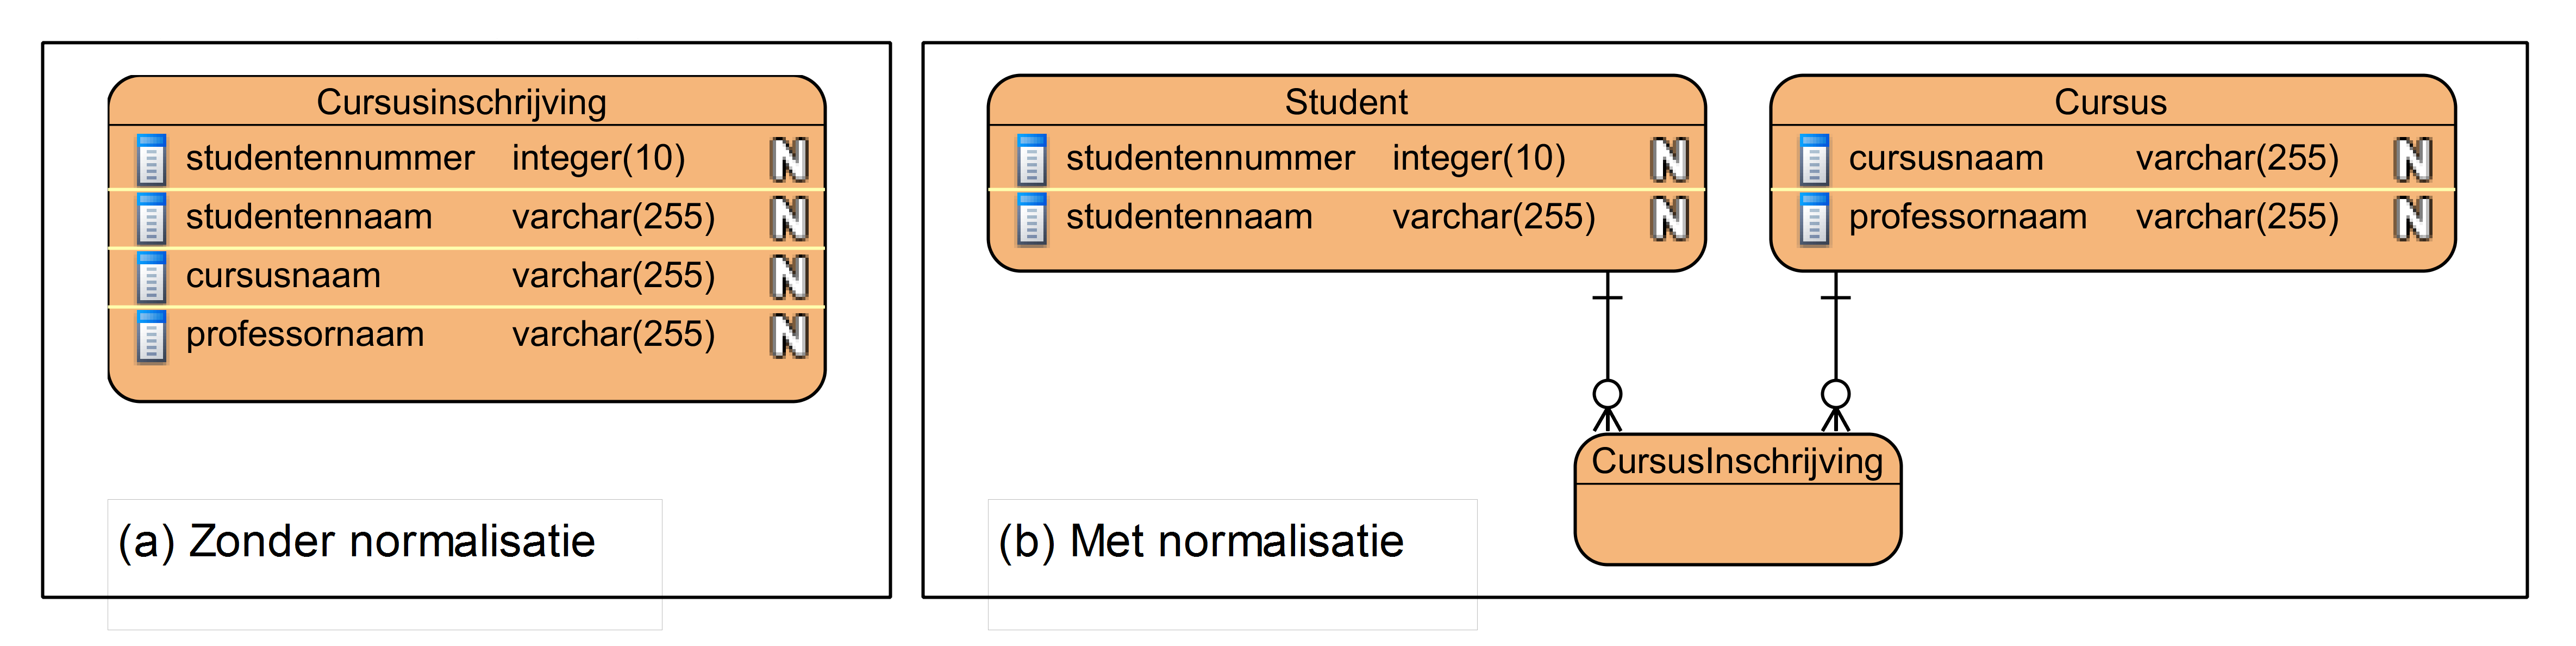
\includegraphics[width=\linewidth]{img/Relationeel-Model-Normalisatie.png}
\caption[Relationeel datamodel (a) zonder en (b) met normalisatie]{Relationeel datamodel (a) zonder en (b) met normalisatie}
\label{fig:Relationeel-Model-Normalisatie}
\end{figure}

Een belangrijk concept in een relationele database is ACID, welk tussen verschillende transacties wordt gegarandeerd:

\paragraph{Atomair (\underline{A}tomicity)} Een database transactie moet oftewel volledig uitgevoerd worden oftewel heeft geen enkele bewerking plaatsgevonden. 

\paragraph{Consistent (\underline{C}onsistency)} Een transactie behoudt de consistentie als de volledige uitvoering van de transactie de database van één consistente staat naar een andere brengt. Een consistente staat is een staat die ervoor zorgt dat waardes van een instantie consistent zijn met de andere waarden in dezelfde staat. Een voorbeeld is het overschrijven van \euro{50} van persoon A naar B, op het einde moet de totale som nog steeds gelijk zijn, A \euro{50} minder en B \euro{50} meer. Een inconsistente staat zou zijn dat enkel A \euro{50} minder heeft maar B nog steeds evenveel. 

\paragraph{Geïsoleerd (\underline{I}solation)} Een transactie moet uitgevoerd worden alsof ze geïsoleerd is van andere transacties, die eventueel gelijktijdig uitgevoerd worden. 

\paragraph{Duurzaam (\underline{D}urability)} Een voltooide transactie kan later niet ongedaan gemaakt worden.

Deze verschillende concepten bieden de gebruiker van het RDBMS garanties die de programmeur van de database kan gebruiken voor zijn systeem. Daartegen over staat wel dat dit de complexiteit van de RDBMS groeit, ook indien dit voor bepaalde toepassingen misschien niet nodig is.

\subsection{NoSQL database}\label{sec:eventualconsistency}
NoSQL DBMS zijn ontstaan als reactie op de 'one size fits all'-gedachte die RDBMS's volgen. Dit is ook zichtbaar in de NoSQL systemen, ze bestaan in verschillende variëteiten, elk met hun eigen eigenschappen en toepassingsgebied. Toch is er een rode draad te vinden tussen de verschillende systemen vergeleken met RDBMS: 
\begin{itemize}
	\item \textbf{Lagere complexiteit}: NoSQL systemen bieden minder opties en features aan dan de RDBMS omdat bepaalde applicaties enkelen nu eenmaal niet nodig hebben. Bijvoorbeeld in een sociale netwerk moet een post niet onmiddellijk beschikbaar zijn voor al de vrienden van een persoon, maar dit mag even duren.
	\item \textbf{Hogere doorvoer}: Talrijke NoSQL systemen bieden een hogere doorvoer van data aan, meestal gecombineerd met een lagere complexiteit. 
	\item \textbf{Horizontale schaalbaarheid en werkend op commodity hardware}: Waar grote RDBMS's draaien op dure high-end systemen, was het bedoeling van NoSQL databases om te werken met eenvoudige machines (commodity hardware). \\
	Horizontale schaalbaarheid staat voor het toevoegen extra machines aan een systeem voor extra resources, in tegenstelling tot verticale schaalbaarheid waar een krachtiger machine wordt gebruikt voor de opschaling. In horizontale opschaling wordt de opschaling gedaan door de data van een enkele database of tabel te verspreiden over verschillende machines die elk maar voor een deel van de data verantwoordelijk zijn en moeten opslaan.\\
	NoSQL systemen combineren deze twee elementen en bieden hierdoor een schaalbaar systeem aan met basis componenten.
	\item \textbf{Datamodel dichter bij objecten}: De meeste NoSQL systemen zijn zodanig ontworpen dat deze de vertaling van objecten naar opslag eenvoudiger of meer gelijkend maken dan RDBMS's. Waar dat RDBMS nog zijn ontworpen voor de object georiënteerde programmeertalen, werd er bij de ontwikkeling van NoSQL onmiddellijk hiermee rekening gehouden.  
\end{itemize}  \noindent
Deze verschillende argumenten leiden vervolgens tot een tegenreactie op ACID, namelijk BASE. \noindent
\begin{itemize}
 \item Basis beschikbaarheid (\textbf{B}asically \textbf{Availability}): het DBMS probeert de data nog steeds beschikbaar te houden, zelf in het geval van één of meerdere falende instanties. 
 \item \textbf{S}oft State: De data moet op een bepaald moment niet volledig consistent zijn. 
 \item Eventuele consistentie (\textbf{E}ventual Consistency): De database zal na enige tijd in een consistente status uitkomen, het is mogelijk dat oudere data tijdelijk leesbaar is. Eventuele consistentie kan op zijn beurt opnieuw onderverdeeld worden in 4 categorieën \cite[slide 16]{lipcon2009design}:
 	\begin{itemize}
 		\item \textit{Read your own writes} consistentie: Ongeachte van de server waarop een gebruiker leest, zal hij zijn update onmiddellijk correct lezen. 
 		\item \textit{Session} consistentie: De gebruiker zal zijn updates onmiddellijk kunnen lezen binnen dezelfde sessie, een sessie is hierdoor meestal gelimiteerd tot een enkele database server. 
 		\item \textit{Casual} consistentie: Als een gebruiker versie X leest en vervolgens versie Y schrijft, zal elke gebruiker die versie Y leest ook versie X lezen.
 		\item \textit{Monotonic Read} consistentie: Dit levert monotone tijdsgaranties dat een gebruiker enkel recentere data versies in de toekomst zal lezen. 
 	\end{itemize}
\end{itemize}
Deze vereisten kunnen gekoppeld worden aan de CAP theorie van Erik Brewer\cite{Brewer:2000:TRD:343477.343502}. CAP zegt dat een gedistribueerd systeem maar twee van de 3 CAP elementen kan ondersteunen: (strikte) consistentie, beschikbaarheid en partitie tolerantie. Met de laatste wordt bedoelt dat enkele instanties van het systeem falen maar er nog steeds een werkend systeem is.  

\subsubsection{Classificatie van NoSQL systemen}
Er zijn vele NoSQL systemen ontworpen gedurende de laatste jaren, elk met hun eigen variëteit, functionaliteit en populariteit. Er bestaan verschillende manieren om de systemen te classificeren, maar één van de meest gebruikte doet dit op basis de data modellering, een korte vergelijking op basis van deze bevindt zich in tabel \ref{table:selectie-classificatie}.  

\begin{table}[!h]
	\resizebox{\textwidth}{!} {
		\begin{tabular}{l l l l l l}
			\textbf{Soort} & \textbf{Performantie} & \textbf{Schaalbaarheid} & 			\textbf{Flexibiliteit} & \textbf{Complexiteit} & \textbf{Functionaliteit} \\ \hline
			Column & hoog & hoog & gematigd & laag & minimaal \\
			Document & hoog & variabel(hoog) & hoog & laag & variabel (laag) \\
			Graph & variabel & variabel & hoog & hoog & graph theory \\
			Key-Value & hoog & hoog & hoog & geen & variabel (geen) \\
		\end{tabular}
	}
	\caption{Classificatie en categorisatie van NoSQL DBMS's door Scofield en Popescu. \cite{categorizatie-sco10} \cite{categorizatie-pop10b} }
	\label{table:selectie-classificatie}
\end{table} 

\paragraph{Column Model}In een column-gebaseerd systeem wordt de data opgeslagen per kolom in plaats van de traditionele manier, per rij. Deze aanpak werd in eerste instantie gedaan voor analyse van business intelligentie. Het systeem is geïnspireerd door de paper van Google’s Bigtable \cite{chang2008bigtable}. \cite{Strauch.NoSQL}

\paragraph{Graph Model} In een grafen model, wordt de data voorgesteld en opslagen volgens de grafen theorie: knopen, lijnen en eigenschappen op de knopen en lijnen. \cite{bollacker2008freebase}.   

\paragraph{Document Model} Document systemen zijn volgens vele de volgende stap in key-value systemen, waar deze complexere structuren toe laten, dit door middel van meerdere key/value paren per element. \cite{Strauch.NoSQL} \\
Een document moet geen vaste structuur hebben maar elk document op zich kan verschillende velden hebben, dit kan bijvoorbeeld toegepast worden bij boeken. Waar een bepaald boek een recept is, kan een ander een deel zijn van een trilogie. Bij het eerste kan de kooktijd opgeslagen worden en bij de tweede een referentie naar de andere boeken. 

\paragraph{Key-Value Model} Key-Value systemen hebben een heel eenvoudig data model, data kan opgeslagen, opgevraagd en verwijderd worden op basis van een key. De informatie die in de database zit, is de waarde voor die key. \\
Met dit eenvoudig model en functionaliteit die weinig complexiteit introduceren, kan er gestreefd worden naar een hoge performantie, schaalbaarheid en flexibiliteit. \cite{Strauch.NoSQL}

\section{Bespreking van verschillende DBMS's}\label{sec:BesprekingDBMS}
De verschillende categorieën databases zijn besproken, voor deze thesis zullen enkele relationele en NoSQL DBMS's in meer detail worden besproken. Databases uit 4 categorieën komen verder aanbod, er is gekozen om de Graph NoSQL DBMS's niet te bespreken omdat deze gericht zijn op andere dataset dan de overige categorieën. 
\begin{itemize}
\item Column NoSQL DBMS's: Cassandra, HBase
\item Document NoSQL DBMS's: Apache CoucheDB, MongoDB
\item Key-Value NoSQL DBMS's: LightCloud (Tokyo), MemCache, Redis, Riak, Project Voldemort
\item Relationele DBMS's: MySQL, Pgpool-II (PostgreSQL)
\end{itemize}

\subsection{Column database}
\subsubsection{Cassandra}
\textit{Website: \url{http://cassandra.apache.org/}}\\
Cassandra is een database systeem die gebaseerd is op 2 verschillende systemen, Amazon's Dynamo en Google's Bigtable, wat voor een combinatie van een column- en key-value-based database zorgt. 

De query taal is beperkt tot 3 operaties: get, insert en delete \cite{Lakshman:2010:CDS:1773912.1773922}, waar de  laatste waarde in geval van een conflict zal opgeslagen worden.

De database kan gedistribueerd uitgerold worden waar door middel van partitionering en een consistent hashing algoritme de data verspreid wordt over de verschillende instanties. Om beschikbaarheid van de data te hebben bij een failure, wordt deze gerepliceerd over verschillende instanties met verschillende configuratie modellen. 

\subsubsection{HBase}
\textit{Website: \url{http://hbase.apache.org/}}\\
HBase is een database systeem die gebaseerd is op Google's BigTable en draait boven op HDFS, Hadoop Distibuted File System.

De query taal voor HBase bestaat uit 4 elementen, een get, put en delete als standaard operaties en een scan om over verschillende rijen te gaan. 

Voor het gedistribueerd draaien van de database, wordt de database ingedeeld in Regions. Vervolgens is een RegionServer verantwoordelijk voor de data van Regions. Daarnaast zijn er nog Zookeeper en Hadoop die respectievelijk verantwoordelijk zijn voor het management van de instanties en de eigenlijke dataopslag.

\subsection{Document database}
\subsubsection{Apache CoucheDB}
\textit{Website: \url{http://couchdb.apache.org/}}\\
Apache CoucheDB is een document database systeem waar alles wordt voorgesteld met behulp van JSON. Het systeem kan bevraagd worden door middel van Map-Reduce, de map gebeurd door een \textit{view}, een JavaScript-functie die de gegevens zal selecteren. Nadien kan met een reduce view de data geaggregeerd worden. 

Bij het gedistribueerd uitrollen zal de data met consistent hashing over verschillende instanties verdeeld worden waar elke instantie dezelfde rol heeft. Nu zal CoucheDB enkel updates van data van instantie veranderen en niet data automatisch verdelen. Ook is het mogelijk om een exacte replica van de ene naar de andere instantie te sturen, dit wordt bijvoorbeeld handig indien documenten naar een laptop gesynchroniseerd worden om later offline te kunnen werken.

In een gedistribueerde omgeving ziet CouchDB conflicten niet als een uitzondering maar als een normale omstandigheid. Wel zullen updates atomisch per rij afgewerkt worden op een enkele instantie, zodat hier geen conflict in kan bestaan. Maar indien een conflict optreedt, is het aan de bovenliggende applicatie om deze af te handelen. 

\subsubsection{MongoDB}
\textit{Website: \url{http://www.mongodb.org/}}\\
MongoDB is een document database systeem waar de data wordt voorgesteld aan de hand van BSON, een binaire vorm vergelijkbaar met JSON. Data kan ingegegeven worden via JSON aangezien er een eenvoudige map mogelijk is. 

Er is een uitgebreide query taal, waar er naast het invoegen, verwijderen en opvragen van een document ook talrijke zoekparameters meegegeven kunnen worden: dit gaat van zoeken op een enkel veld tot conjuncties, sorteren, projecties, ... 

MongoDB kan in een gedistribueerde omgeving opgezet worden met een opsplitsing tussen het redundant opslaan van data en het verdelen van data. Het redundant opslaan wordt toepast door het combineren van instanties in een ReplicaSet waar er een master-slave configuratie is. Daarnaast kan data ook verdeeld worden over verschillende instanties of replica sets, dit kan door middel van het configureren van shards. 
Conflicts worden opgevangen door de master waar er telkens een meerderheid van de instanties nodig is om deze te verkiezen. 

\subsection{Key-Value database}
\subsubsection{LightCloud (Tokyo)}
\textit{Website: \url{http://opensource.plurk.com/LightCloud/}}\\
LightCloud is een gedistribueerde uitbreiding van Tokyo Tyrant. Tokyo Tyrant is op zijn beurt een uitbreiding op Tokyo Cabinet en voegt de mogelijkheid tot externe connecties aan Cabinet toe. Cabinet is het basis pakket. 

De query taal is gelimiteerd tot 5 operaties: get, put, delete, add en een iterator om over de keys te gaan. Met add wordt er data aan een bestaand element toegevoegd. 

LightCloud levert een gedistribueerde database met master-master synchronisatie. Met behulp van een consistent hashing algoritme en 2 hash rings, wordt de data verdeeld over verschillende instanties met de nodige redundantie. De eerste ring is verantwoordelijk voor de lookups oftewel het lokaliseren van de keys, de storage ring is verantwoordelijk voor het opslaan van de verschillende waarden. 

\subsubsection{MemCache}
\textit{Website: \url{http://memcached.org/}}\\
MemCache is een veel gebruikt systeem waarin al de data in RAM geheugen wordt gehouden en alhoewel er ondersteuning is met behulp van MemCacheDB voor persistentie is deze database niet bedoeld voor persistente opslag. 

De query mogelijkheden zijn beperkt tot get, put en delete van een waarde. In het geval een key meerdere keren geschreven wordt, zal de laatste waarde teruggegeven worden. 

\subsubsection{Redis}
\textit{Website: \url{http://www.redis.io/}}\\
Redis is een key-value database met de mogelijkheid tot opslaan van complexe datastructuren zoals lijsten, sets en mappen. Naast de standaard instructies om een enkele waarde toe te voegen, zijn er specifieke commando's om operaties op de complexere objecten te doen. Redis biedt ook ondersteuning voor transacties en heeft deze de mogelijkheid tot expire, hierdoor zal een waarde automatisch vergeten worden na een meegegeven tijd. 

De database wordt volledig in geheugen geplaatst maar ondersteunt 2 soorten van persistentie, oftewel door middel van RDB, oftewel met een AOF log. Bij RDB worden er over tijd snapshots gemaakt van de database en weggeschreven op harde schijf. In het geval van AOF wordt elke schrijfoperaties weggeschreven en kan de database opgebouwd worden met behulp van deze lijst.

Tenslotte heeft Redis momenteel een relatief beperkte mogelijkheid tot een gedistribueerde database. Het is mogelijk om data over verschillende instanties te distribueren met behulp van sharding welke op voorhand gedefinieerd dient te worden en is er ook de mogelijkheid tot master-slave opstelling met automatische failure detection.
De laatste is nog wel in beta, al is het mogelijk om deze te gebruiken. Tenslotte is er in de toekomst meer ondersteuning op komst met behulp van Redis Cluster waar data automatisch verspreid wordt over verschillende instanties. 

\subsubsection{Riak}
\textit{Website: \url{http://basho.com/riak/}}\\
Riak is een key-value database met de mogelijkheid tot opslaan van strings, JSON en XML. Daarnaast heeft deze standaard operaties maar hier enkele uitbreidingen op gemaakt. Allereerst is het mogelijk om secundaire indexen te definiëren op de elementen, MapReduce toe te passen en een full-text search. 

Riak is gebouwd om gedistribueerd te draaien waar al de instanties evenwaardig zijn. Data wordt verdeeld over de verschillende instanties en elk element wordt standaard op 3 verschillende instanties opgeslagen. Indien een bepaalde instantie faalt, wordt dit met een gossiping algoritme verspreid over de verschillende instanties waarmee een naburige instantie overneemt. Daarnaast is er automatische recovery indien een instantie terug online komt. 

\subsubsection{Project Voldemort}
\textit{Website: \url{http://www.project-voldemort.com/}}\\
Project Voldemort is een key-value store met enkel 3 basis operaties: get, put en delete met de mogelijkheid voor als keys en values strings, serializable objecten, protocol buffers of raw byte arrays te gebruiken. 

Deze database ondersteunt verschillende modes van distributie. De opbouw bestaat uit verschillende lagen, elk met hun eigen gedefinieerde functie. Met behulp van deze lagen kan de ontwikkelaar extra functionaliteit toevoegen met behulp van een extra laag om de applicatie meer te finetunen naar zijn uitwerking. 
Data wordt verdeeld met behulp van consistent hashing over de verschillende servers, waarbij data verschillende keren wordt bijgehouden om ervoor te zorgen dat de data nog beschikbaar is in het geval van falen. 

\subsection{Relationele database}
\subsubsection{MySQL}
\textit{Website: \url{http://www.mysql.com/}}\\
MySQL is een relationele database waarin data kan voorgesteld worden in verschillende vormen, beginnend met een bool tot een blok tekst. Daarnaast zijn de query mogelijkheden uitgebreid. 

De uitbreiding van een gedistribueerd systeem is bij MySQL ingebouwd door middel van een Master-Slave configuratie. Als mysqlfailover een faal detecteert in één van de slaven, zal de database verder werken, bij het falen van de master zal een nieuwe master handmatig aangeduid moeten worden. Ook de recovery moet handmatig gestart worden, waarna indien gewenst de originele master opnieuw als master kan gezet worden (bv. omdat deze de krachtigste computer is). 

\subsubsection{Pgpool-II (PostgreSQL)}
\textit{Website: \url{http://www.pgpool.net/}}\\
PostgreSQL is een relationele database en heeft soortgelijke specificaties als MySQL op een enkele computer, verschillende soorten data kunnen voorgesteld worden met uitgebreide query mogelijkheden. 

Enkel als de database ook gedistribueerd moet uitgerold worden, is er een verschil. Bij PostgreSQL is er standaard geen ondersteuning hiervoor maar moet er op externe elementen vertrouwd worden. Er bestaan verschillende componenten soorten systemen, maar het meeste uitgebreide pakket is Pgpool-II. Deze ondersteund load-balancing, een vergelijking van de systemen kan gevonden worden op de wiki van PostgreSQL \cite{postgresql-clustering}. 

Pgpool-II heeft verschillende mode, zoals parallel mode waar de data verdeeld wordt over verschillende instanties of replicatie waar de data op meerdere instanties wordt opgeslagen zodat deze nog beschikbaar is bij het falen van een enkele instantie.

\subsection{Conclusie} 
Deze 10 systemen laten een variatie van verschillende opties zien, zowel in query mogelijkheden als naar een gedistribueerde configuratie waar er keuzes volgens het CAP theorema gemaakt moeten worden. 

Bij het kiezen van een systeem is het moeilijk om een keuze te maken af en toe, in het volgend gedeelte zal er besproken worden wat er momenteel beschikbaar is als resultaten of te gebruiken tool. 

\section{Objectieve vergelijking van de verschillende systemen volgens CAP}
De databasemanagementsystemen zijn voor meer dan 40 jaar actief. Met de opkomst van het relationele model in 1969 door E. Codd \cite{Codd:1970:RMD:362384.362685}, zijn gedurende vele jaren de relationele DMBS de leidende technologie geweest. Maar de afgelopen 10 jaar is er in het landschap veel veranderd met de opkomst van de NoSQL DBMS's die afstappen van het ACID naar BASE, meer gefocust op het werken op grote data in een gedistribueerde omgeving. 

Nu zijn er vele verschilpunten tussen verschillende systemen, dit gaat van het datamodel tot de verschillende keuzes in het CAP theorema. In dit gedeelte zal er gekeken worden welke methodes er al beschikbaar zijn voor het meten van de performantie, consistentie en beschikbaarheid en mogelijke resultaten. 

\subsection{Performantie benchmarking}
Indien men verschillende DBMS wilt vergelijken bestaan er al enkele tools en studies om de performantie te kunnen vergelijken, een blogpost van A. Popescu \cite{PopescuBenchmarkOverview} geeft een overzicht van verschillende benchmarking tools. 

Als eerste hebben vele DBMS's interne benchmarking tools, waarmee de database op verschillende configuraties kan getest worden en vergeleken worden. Deze resultaten zijn nuttig indien het DBMS al gekozen is en men bezig is met het aanpassen van de parameters of om te onderzoeken wat net de bottleneck is in een bepaald systeem. Een voorbeeld hiervan is mongoperf\footnote{\url{http://docs.mongodb.org/manual/reference/program/mongoperf/}} voor MongoDB. 

Andere studies focussen op het testen van verschillende systemen en daarbij kunnen verschillende doelstellingen zijn: het ontwikkelen van een breed toepasbare tool, het testen van een grote verscheidenheid van DBMS's of het testen van een specifieke categorie van systemen. Elke van deze benchmarking brengt extra kennis bij maar heeft ook zijn beperkingen. Het totaal pakket van al de testen kan een gebruiker de informatie geven om een beter gefundeerde keuze te maken. 

De eerste categorie, het \textbf{ontwikkelen van een tool}, heeft als grote voordeel dat andere gebruikers nadien de testen opnieuw kunnen uitvoeren met de huidige systemen. Het is namelijk niet gegarandeerd dat het resultaat van een jaar geleden met de nieuwste versie nog te vergelijken is.
Het grootste nadeel is het type testen dat kan uitgevoerd worden, er is een grote variëteit aan systemen elk met hun eigen datastructuur en query mogelijkheden. De tool moet dus een gemeenschappelijke subset zoeken en enkel dit soort queries kunnen getest worden. Een voorbeeld van een dergelijke tool de opensource tool YCSB\cite{cooper2010benchmarking}. In deze tool kan elk DBMS's getest worden zolang een basisset van 5 queries kan implementeren: het invoegen, updaten, verwijderen en opvragen van een enkel record met daarnaast ook de mogelijkheid tot range queries, met behulp van 1 query een verzameling van records tegelijk op te vragen. \\
Sommige systemen ondersteunen bepaalde queries niet onmiddellijk maar bevatten wel de functionaliteit om deze via een omweg te implementeren, bijvoorbeeld een update kan geïmplementeerd worden door het opvragen, verwijderen en vervolgen invoegen van de geüpdatete record. 

Een volgende categorie zijn de \textbf{resultaten van gerelateerde DBMS's}, in deze categorie zijn er voornamelijk resultaten te vinden van systemen met hetzelfde datamodel. Het grote voordeel hieraan is dat deze systemen in de meeste gevallen een vrij gelijkaardige set aan query mogelijkheden bevatten waardoor er meer diepgang is dan tussen meer verschillende systemen. Een voorbeeld van zulk onderzoek is gedaan door P. Pirzadeh et al\cite{pirzadeh2011performance} voor de key-value systemen, meer specifiek is er gefocust op het uitvoeren van range queries tussen Cassandra, HBase en Voldemort. Hoewel in de categorisatie van deze thesis de eerste twee onder column NoSQL vallen, zijn deze nog vrij gelijklopend. \\
In deze categorie vallen ook de resultaten die meestal getoond worden op de website van de DBMS's, een vergelijkende benchmark met andere soortgelijke systemen. Hoewel de resultaten niet altijd volledig objectief zijn, kan de gevolgde test methode wel interessant zijn. Een voorbeeld van deze studie is de Key-Value benchmarking van VoltDB\cite{huggkey} waar Cassandra en VoltDB vergeleken worden, een belangrijke kanttekening is dat de auteur zelf al aanhaalt dat de systemen vrij verschillend zijn zoals appels en appelsienen.  

Als laatste categorie, zijn er de \textbf{resultaten van verschillende DBMS's} waar zeer verscheidene systemen met elkaar getest worden. De belangrijkste voordeel is dat er resultaten zijn die verschillende soorten met elkaar vergelijken en waardoor niet alleen verschillen in het datamodel kunnen vergeleken worden in toekomstige studies maar ook performantie verschillen. Het nadeel is ook hier dat er een gemeenschappelijke subset gevonden moet worden, hierdoor kunnen bepaalde databases hun kracht net niet laten zien. Verschillende van deze onderzoeken zijn \cite{tudorica2011comparison} en \cite{rabl2012solving}. Deze laatste maakt gebruik van de YCSB tool die hierboven besproken was. 


\subsection{Consistentie testen}
Zoals besproken in het vorige gedeelte, is er al relatief veel onderzoek gebeurd naar de performantie van de verschillende systemen. Maar daarnaast is er ook de consistentie eigenschappen die verschillend kunnen zijn. 

Een recent artikel \cite{golab2014eventually} (maart 2014), begint met het stellen dat er momenteel nauwelijks gekwantificeerde methodes bestaan om de eventuele consistente te meten. In hun artikel stellen zijn mogelijke methoden voor: de actieve of passieve analyse. \\
De \textbf{actieve} analyse bestaat het wegschrijven van data in een database waarna 1 of meerdere andere gebruikers meten hoe lang het duurt vooraleer zij de nieuwe waarde lezen. 
De \textbf{passieve} analyse wordt er gekeken hoe de gebruiker interageert met het systeem en hoe de data updates zich gedragen. Leest deze altijd de laatste waarde (=strikte consistentie)? Is het mogelijk dat een nieuwe waarde al wordt gelezen voor de schrijfactie voltooid is? \\
Beide systemen hebben hun eigenschappen, de actieve analyse kan gezien worden als een systeem georiënteerde analyse en test hoe lang het duurt voor de data beschikbaar is over de verschillende systemen en heeft als uitkomst hoe DBMS's zich verschillend gedragen ten opzichte van elkaar of in verschillende netwerk- en hardwareomgevingen. 
Bij de passieve analyse is georiënteerd naar de gebruiker toe, hoe moet deze zijn toepassingen aanpassen, wat zijn specifieke eigenschappen van het systeem? 

Voor beide analyse methodes is er al onderzoek gebeurd, maar het meeste is gebeurd naar de actieve analyse. Onder andere Duitse onderzoekers hebben op het Amazon S3 platform getest hoe lang het duurt vooraleer data geschreven in MiniStorage, een database systeem, beschikbaar is voor alle gebruikers. \cite{bermbach2011eventual}. \\
Daarnaast zijn er ook 2 interessante resultaten gevonden: allereerst heeft het Amazon S3 systeem geen monotone lees consistentie, daarnaast bleek het inconsistentie interval voor een bepaald record periodiek verloop te hebben dat niet door de onderzoekers verklaard konden worden. 

De YCSB software van hierboven is door onderzoekers in de VS uitgebreid naar YCSB++\cite{patil2011ycsb++} waardoor deze meer ondersteuning heeft om het meten van systeembelasting maar ook voor de consistentie eigenschappen. Hoewel enkele van de systemen die zij testen in principe strikt consistent zijn zoals HBase, worden deze eventueel consistent door het gebruiken van buffers bij de gebruiker. Vervolgens testen zij hoe lang het duurt voor de data ook gelezen kan worden. Een probleem met deze methode is dat deze vertraging sterk afhankelijk is van het aantal acties van de schrijvende gebruiker: indien er meer geschreven wordt, zal de buffer sneller verzonden worden naar de server en dus sneller beschikbaar zijn voor andere gebruikers. \\
Hoewel zij stellen dat er ook testen zijn gedaan naar eventuele consistentie voor Cassandra en MongoDB, zijn de resultaten niet beschikbaar in het artikel of op de website. 

Andere onderzoeker\cite{wada2011data} hebben passieve analyse uitgevoerd en gekeken hoe lang het duurt vooraleer databases in de cloud infrastructuur consistente data hebben, met een focus op Amazon SimpleDB. Er zijn testen uitgevoerd hoe lang het duurt vooraleer de meest recente data gelezen zal worden door een gebruiker. 

Bij Netflix heeft men aan passieve analyse gedaan op hun Cassandra systeem \cite{kalantzisnetflix} waar zij in hun testen geen consistentie problemen vonden naar de gebruiker toe. Er is geen vermelding hoeveel vertraging er zit tussen beide transacties. Volgens hun gaat het meer om de perceptie dat data verkeerd kan gelezen worden en de angst van het middle management. 

\subsection{Beschikbaarheidstesten}
Een derde verschilpunt is hoe de systemen omgaan met het falen van een enkele server en dit onder verschillende opties: Het is mogelijk dat deze tijdelijk uitgeschakeld wordt wegens onderhoudt, het kan om een onverwachte crash van het DBMS's gaan of zelfs een hele server, tenslotte kunnen er ook nog netwerkproblemen optreden waardaar deze (tijdelijk) niet beschikbaar is. 

Nu hoe gaan deze systemen om het falen en terug online brengen van de systemen: zijn er geen acties mogelijk op de server, worden de connecties tijdelijk verbroken, is er een verhoogde of verlaagde vertraging op de transacties? En detecteert het systeem automatisch wanneer de oorspronkelijke server terug online komt of moet gemeld worden om de server terug te gebruiken? In een NoSQL DBMS waar gewerkt wordt commodity hardware, zal het falen regelmatig gebeuren en verschillende systemen reageren anders op deze acties. 

Voor informatie over hoe de verschillende systemen reageren, is het momenteel uitzoeken op de website van de software verdeler en zelf uittesten van het gedrag. Naar mijn onderzoek, bestaat er nog geen vergelijkende studie tussen de verschillende systemen. 

\section{Conclusie}
Na het artikel van E. Codd \cite{Codd:1970:RMD:362384.362685} in 1969, heeft het relationele model een dominante rol gespeeld in het database model. Met de opkomst van het internet, grotere hoeveelheden data en steeds complexere RDBMS's, is er een nieuwe stroming gekomen in de database wereld, de NoSQL DBMS's. Deze beloven betere schaalbaarheid, hogere performantie en dit op commodity hardware ten aanzien van de \gls{acid} eigenschappen naar \gls{base}: een hogere beschikbaarheid en eventuele consistentie.  

In deze thesis zal er eerst een algemene methode voorgesteld worden om verschillende systemen te testen naar de eventuele consistentie, behandelen van storingen (failure handling) en (automatisch) herstel (automatic recovery).  \\
Daarna zal deze methode uitgevoerd worden op verschillende databases waar verschillende resultaten en opvattingen gezien kunnen worden. Deze leiden tot enkele initiële conclusies die in de toekomst verder kunnen worden onderzocht. 